\subsubsection{Overview}
\label{Spike-triggered Average}
\index{Spike-triggered Average}\index{utilities, Spike-triggered Average}

\begin{figure}[h]
\begin{center}
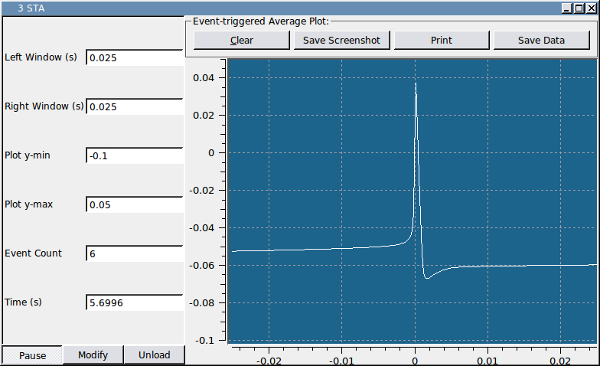
\includegraphics[width=4in]{spiketriggeredaverage.png} 
\caption[Spike-triggered Average]{This module computes an event or spike-triggered average of any input signal.} 
\end{center}
\label{spiketriggeredaverage}
\end{figure}

This module computes an event or spike-triggered average of any input signal. You specify a time window of interest around the spike. This screenshot was made using a neuron model to generate spikes and the SpikeDetect module to detect spikes. The STA module then plots the average spike shape waveform is plotted.

This module required the Boost libraries, which can be installed in Ubuntu by running:
\begin{example}
\$ sudo apt-get install libboost-dev
\end{example}

\subsubsection{Input Channels}
\begin{description}
\item[input(0) - Input] quantity to compute the spike-triggered average for
\item[input(1) - Event Trigger] trigger that indicates the spike time/event (=1)
\end{description}

\subsubsection{Output Channels}
\begin{description}
\item[output(0) - Isyn] output current (A)
\end{description}

\subsubsection{Parameters}
\begin{description}
\item[Left Window (s)] Amount of time before the spike to include in average
\item[Right Window (s)] Time after spike to include in average
\item[Plot y-min] Set minimum for y-axis in the plot
\item[Plot y-max] Set the y-axis maximum
\end{description}

\subsubsection{States}
\begin{description}
\item[Event Count] Number of spikes (event) that are included in the current average
\end{description}